\documentclass{article}

\usepackage{graphicx}
\graphicspath{ files\ }

\title{Tarea01}
\author{Angel Christian Pimentel Noriega}

\begin{document}
\maketitle

\section{Definicion del Problema}
Usando una web api(Open Weather) solicita el clima de 6000 vuelos comerciales, en sus ciudades de origen y de destino

\section{Analisis del Problema}
Requisitos de entrada:\\
Un archivo .csv separado por comas
  Una conexion a internet estable
\\Salida:\\
La salida consiste en un String con el nombre de la ciudad su clima y su temperatura.\\
La forma en que se soluciono el problema fue asi:\\
Creando un objeto reader el que leera el archivo csv con el modulo csv de python\\
Se crea un diccionario el cual actuara comoun cache para evitar solicitudes duplicadas\\
En cada renglon del archivo se lee y si no existen las ciudades en el diccionario se crea un nuevo
objeto ciudad.\\
Este objeto ciudad recibe como parametros latitud y longitud con estos creara una peticion a Open Weather\\
La peticion se crea en el modulo "petition" que trata el JSON recibido de la peticion y regresa un string con 
el clima de la ciudad junto con su temperatura.\\
Finalmente se imprime cada ciudad con el string recibido de "petition"
\section{Seleccion de la mejor alternativa}
Lenguaje de programacion: Python\\
Modulos requeridos: "csv","requests","sys"
\section{Diagrama de flujo}
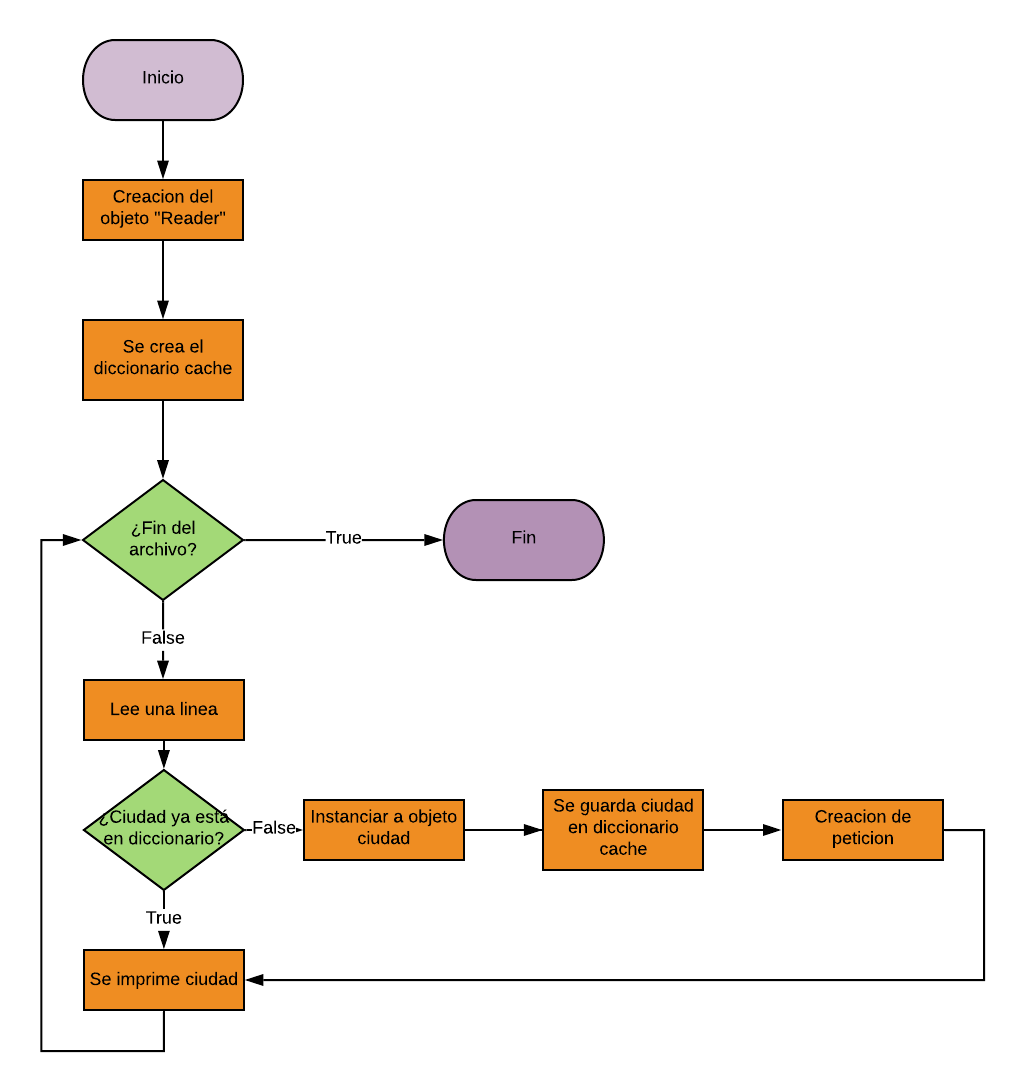
\includegraphics{Imagen.png}
\section{Mantenimiento}
El mantenimiento que este programa necesitaria seria la actualizacion de la api-key si el programa
llegara a necesitar mas peticiones por dia\\
Tambien si Open Weather llegara a cambiar la forma en la que sus solicitudes son creadas\\
Cobraria por el \$2500 por la instalacion y \$100 mensual de mantenimiento

\end{document}
